% !TEX root = ../thesis.tex

\chapter{Hintergrund}

\paragraph{Ausblick:}
Zum besseren Verständnis der weiteren Verlaufs dieser Arbeit, dient dieses Kapitel zur Einführung in die zugrundeliegenden Themen. Dazu wird zunächst die featurebasierte Softwareentwicklung erläutert, ehe dann der Themenbereich des Machine Learnings vorgestellt wird. Dazu werden die Klassifikation und die Fehlervorhersage mittels Machine Learning erläutert. Unterstützt werden die Abschnitte von Grafiken zum besseren Verständnis der Zusammenhänge.
\\
\hrule

\section{Featurebasierte Softwareentwicklung}

\section{Machine-Learning-Klassifikation}

\textbf{ÜBERARBEITEN!}

Die Machine-Learning-Klassifikation unterliegt dem Teilgebiet des \emph{überwachten Machine Learnings} (englisch: supervised Machine Learning). Die nachfolgende \autoref{fig:ml} präsentiert den allgemeinen Prozess des überwachten Machine Learnings auf vereinfachter Weise anhand eines Beispiels. Anhand dieser werden die wichtigsten Informationen zum genannten Themengebiet erläutert. 

\begin{figure}[H]
    \centering
    \captionsetup{justification=centering,margin=2cm}
    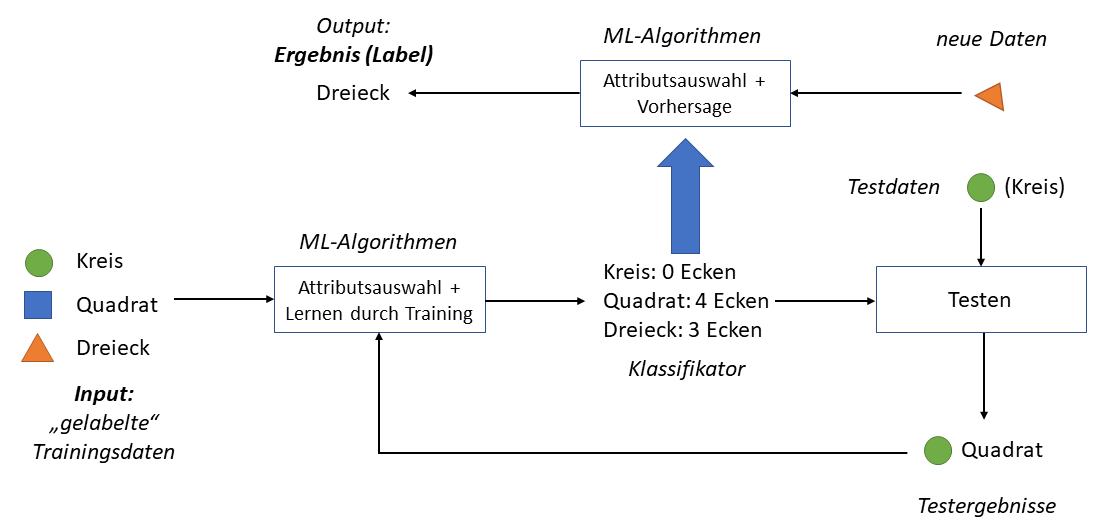
\includegraphics[width=\textwidth]{images/ML}
    \caption{Allgemeiner Prozess des überwachten Machine Learnings dargestellt anhand eines Beispiels (vereinfacht)}\label{fig:ml}
\end{figure}

Das in der Abbildung gezeigte Beispiel zeigt den Prozess der Entwicklung und Anwendung eines Klassifikators zur Erkennung von geometrischen Formen.
Der Prozess beginnt mit der Erstellung eines Datensets, welches als Input für die Anlernung des Klassifikators dient.

\textbf{ÜBERARBEITEN!}

\begin{figure}[H]
    \centering
    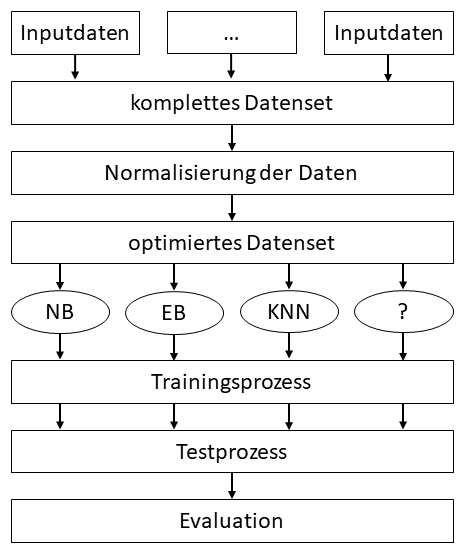
\includegraphics[width=0.5\textwidth]{images/Prozess}
    \caption{Angewendeter Prozess zur Durchführung der Klassfikation nach \cite{Ceylan2006}}\label{fig:process}
\end{figure}

\section{Fehlervorhersage mittels Machine Learning}

Die nachfolgenden drei Abbildungen zeigen den von Queiroz et at. \cite{Queiroz2016} angewandten Prozess zur Entwicklung und Anwendung eines featurebasierten Klassifikators im Rahmen des überwachten Machine Learnings. Die gezeigten Darstellungen orientieren sich sowohl gestalterisch als auch inhaltlich an den in \autoref{fig:ml} gezeigten allgemeinen Prozess des überwachten Machine Learnings. Ferner dient dieser Prozess als grundlegender Prozess für diese Arbeit.

\begin{figure}[H]
    \centering
    \captionsetup{justification=centering}
    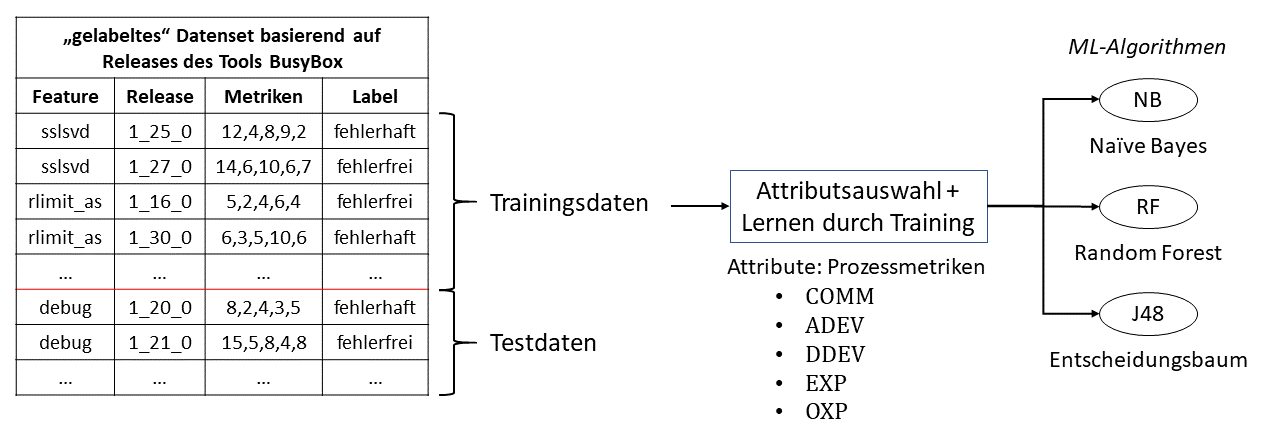
\includegraphics[width=\textwidth]{images/ML1}
    \caption{Teil 1: Featurebasierter Prozess des überwachten Machine Learnings nach \cite{Queiroz2016}}\label{fig:ml1}
\end{figure}

Die Datenbasis des Datensets bilden Commits des UNIX-Toolkits BusyBox\footnote{\url{https://busybox.net/}}, dessen Quellcode frei verfügbar in einem Git-Repository\footnote{\url{https://git.busybox.net/busybox/}} eingesehen und von dort geklont werden kann. Diese Commits wurden wiederum ihren entsprechenden Releases zugeordnet, welche auf der vergebenen Tag-Struktur des Repositories beruhen. Ferner wurden aus den Diffs der Commits die dort bearbeiteten Features extrahiert und anschließend zusammen mit den Release-Informationen in einer MySQL-Datenbank gespeichert. Zusätzlich enthält jeder Datenbankeintrag aggregierte Werte von fünf auf das Feature und den Release bezogenen Prozessmetriken (Erläuterung folgt), sowie das binäre Label, ob ein Feature in einem Release fehlerhaft oder fehlerfrei war. Ein Feature gilt in einem Release als fehlerhaft, sofern in einem Commit des darauffolgenden Releases ein fehlerbehebender Commit festgestellt werden konnte. Dies geschieht über die Analyse der Commit-Nachrichten. Sofern eine Commit-Nachricht die Begriffe "Bug", "Error", "Fail" oder "Fix" enthält, werden die Autoren des Papers den Commit als fehlerbehebend. Wie im Rahmen des überwachten Machine Learning üblich, wird das Datenset in Trainings- und Testdaten in einem Verhältnis von 75:25 geteilt. 

Die Trainingsdaten werden dann den Klassifikatoren zur Anlernung zur Verfügung gestellt. Als Attribute dienen die fünf bereits erwähnten Prozessmetriken. Die nachfolgende Tabelle gibt einen Überblick über die Beschreibungen dieser.

\begin{table}[H]
\centering
\caption{Übersicht der verwendeten Prozessmetriken}
\label{tab:metrics}
\begin{tabular}{l|l}
\textbf{Metrik} & \textbf{Beschreibung}                                                                                                                                                                         \\ \hline
COMM            & \begin{tabular}[c]{@{}l@{}}Anzahl der Commits, die in einem Release dem betreffenden \\ Feature / der betroffenen Datei gewidmet sind\end{tabular}                                            \\
ADEV            & \begin{tabular}[c]{@{}l@{}}Anzahl der Entwickler, die das betreffende Feature / \\ die betreffende Datei in einem Release bearbeitet haben\end{tabular}                                       \\
DDEV            & \begin{tabular}[c]{@{}l@{}}kummulierte Anzahl der Entwickler, die das betreffende Feature /\\ die betreffende Datei in einem Release bearbeitet haben\end{tabular}                            \\
EXP             & \begin{tabular}[c]{@{}l@{}}Geometrisches Mittel der "Erfahrung" aller Entwickler, die am \\ betreffenden Feature / an der betreffenden Datei in einem Release\\ gearbeitet haben\end{tabular} \\
OEXP            & \begin{tabular}[c]{@{}l@{}}"Erfahrung"des Entwicklers, der am meisten zum betreffenden \\ Feature / zur betreffenden Datei in einem Release beigetragen hat\end{tabular}                     
\end{tabular}
\end{table}

\begin{figure}[H]
    \centering
    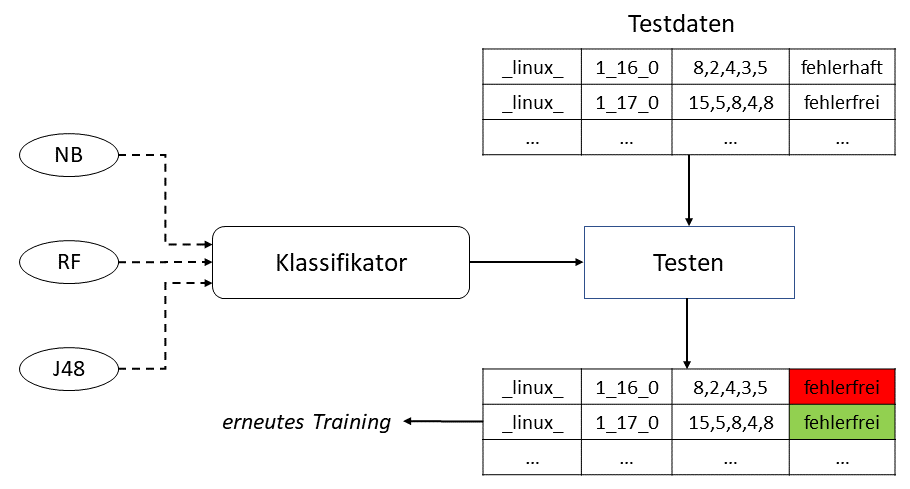
\includegraphics[width=\textwidth]{images/ML2}
    \caption{Teil 2: Featurebasierter Prozess des überwachten Machine Learnings nach \cite{Queiroz2016}}\label{fig:ml2}
\end{figure}

\begin{figure}[H]
    \centering
    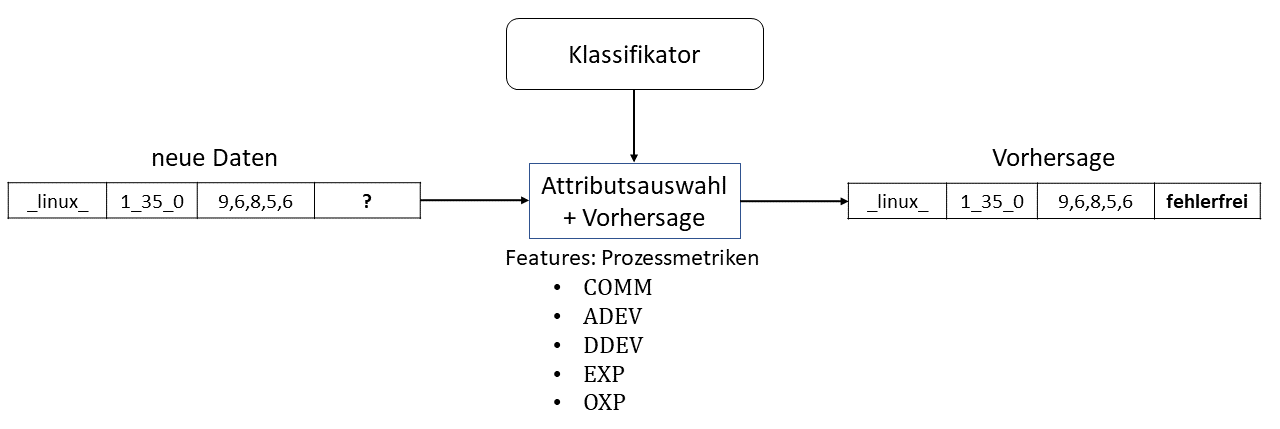
\includegraphics[width=\textwidth]{images/ML3}
    \caption{Teil 3: Featurebasierter Prozess des überwachten Machine Learnings nach \cite{Queiroz2016}}\label{fig:ml3}
\end{figure}

\cleardoublepage
